\documentclass[12pt,letterpaper]{hmcpset}
\usepackage[margin=1in]{geometry}
\usepackage{graphicx}
\usepackage{hyperref}

% info for header block in upper right hand corner
\name{ }
\class{Math 65}
\assignment{HW 11}
\duedate{Wednesday, June 1, 2016}

\newcommand{\m}[1]{\begin{bmatrix}#1\end{bmatrix}}
\newcommand{\f}[2]{\frac{#1}{#2}}
\newcommand{\pn}[1]{\left(#1\right)}
\newcommand{\abs}[1]{\left|#1\right|}
\newcommand{\bk}[1]{\left|ft[#1\right]}
\renewcommand{\bf}[1]{\mathbf{#1}}
\renewcommand{\labelenumi}{{(\alph{enumi})}}

\begin{document}

\problemlist{1, 2, 3, 4, 5}

\begin{problem}[1]
    Consider the planar autonomous system 
    \begin{align*}
        x'(t)&=1-y^2\\
        y'(t)&=1-x^2
    \end{align*}
    \begin{enumerate}
        \item What are the $x$- and $y$-nullclines of the DEs?  Use
            these nullclines to determine the regions of the plane in
            which the solution orbits would be moving left, right, up,
            and down.
        \item Locate all the equilibrium points of the system by
            finding the intersections of the nullclines.
        \item Print out a phase plane portrait of the DE in the
            rectangle $|x|\leq3,|y|\leq3$ using either
            pplane\footnotemark or ODEToolkit\footnotemark.
            Explain how this phase plane portrait is consistent with all
            of the observations you've made on this problem.
        \item For each equilibrium point you found in part (b), use
            the phase plane portrait to determine if it looks like it is
            asymptotically stable, neutrally stable or unstable, and
            whether you have a node, saddle point, or spiral of some
            sort.
    \end{enumerate}
    \footnotetext{\textsuperscript{1}\url{
        http://math.rice.edu/~dfield/dfpp.html}}
    \footnotetext{\textsuperscript{2}\url{http://odetoolkit.hmc.edu}}
\end{problem}
\begin{solution}
    \vfill
\end{solution}
\newpage

\begin{problem}[2]
    Here's a phase plane portrait for a planar, autonomous system of
    DEs. Find a system of DEs that matches this phase plane portrait
    as best as you can. Use software to print out your phase plane
    portrait. Explain thoroughly (using nullclines, where the
    solutions are moving left/right/up/down, equilibrium points) why
    your system of DEs matches the given phase plane portrait.
    \begin{center}
        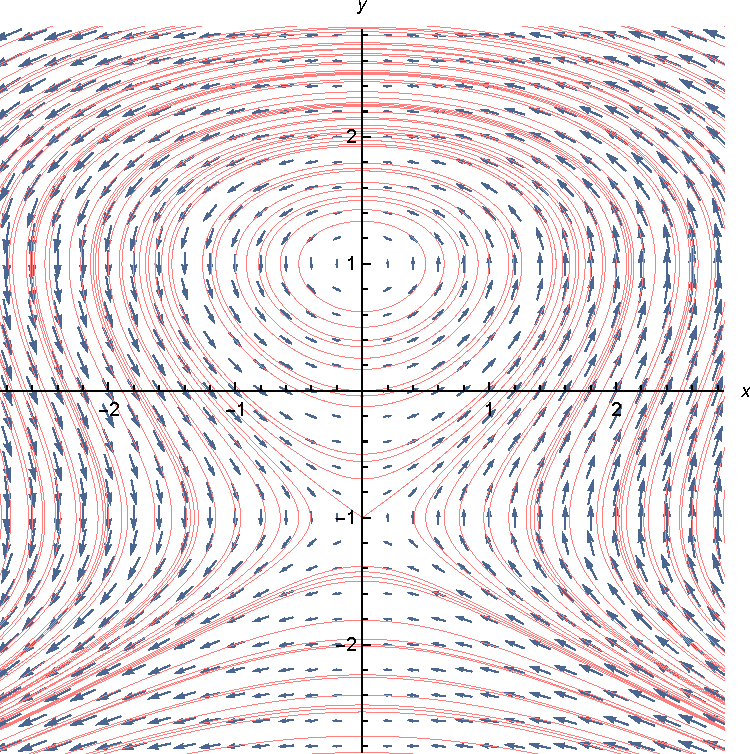
\includegraphics[scale=0.8]{img/june_1_2}
    \end{center}
\end{problem}
\begin{solution}
    \vfill
\end{solution}
\newpage

\begin{problem}[3]
    Consider the linear, constant-coefficient, homogeneous
    differential equation system
    \[
        \bf{x}'(t)=\m{x'(t)\\y'(t)}=\m{a&b\\c&d}\m{x(t)\\y(t)}.
    \]
    Pick values of $a, b, c, d$ so that the equilibrium point at the
    origin is
    \begin{itemize}
        \item an unstable saddle point,
        \item an improper node (asymptotically stable or unstable,
            your choice),
        \item a center (neutrally stable), and
        \item a spiral (asymptotically stable or unstable, your
            choice).
    \end{itemize}
    Use software to print out a phase plane portrait for each case. On
    top of your portrait, plot the nullclines and show that solution
    curves cross them in the proper way.
\end{problem}
\begin{solution}
    \vfill
\end{solution}
\newpage

\begin{problem}[4]
    A $m$~kg mass is suspended at the end of a (massless) rod with
    length $L$~meters. The other end of the rod is fixed at a pivot
    point. This arrangement leads to a simple pendulum that
    swings in a plane. Let $\theta(t)$ be the angular position of the
    pendulum, measured so that the resting position of the pendulum
    corresponds to $\theta=0$ and positive $\theta$ is in the
    direction of the arrow below.
    \begin{center}
        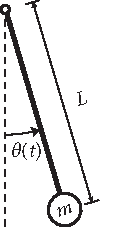
\includegraphics{img/june_1_4}
    \end{center}
    There are two forces acting on the pendulum: gravity and
    friction. You may assume that the friction (due to air resistance
    or friction in the pivot) causes a torque that is proportional to
    the angular velocity, $\dot{\theta}$.
    \begin{enumerate}
    \item First, derive a governing equation using the rotational
        analog of Newton's second law, $\tau=I\ddot{\theta}$.  (See
        Chapter 18 of your Physics 24 textbook.) You can assume that the
        mass is concentrated at a point and the rod is massless, so the
        moment of inertia of the mass is $I=mL^2$.  You should obtain
        the differential equation
        \[
            \ddot{\theta}+c\dot{\theta}+\f{g}{L}\sin\theta=0.
        \]
        What must be the units of the damping constant $c$?
    \item Write your second-order differential equation as a system of
        first-order equations by defining
        $\omega(t)=\dot{\theta}(t)$. Are they linear or nonlinear?
        Autonomous or nonautonomous?
    \item Locate the equilibrium points of this system. (There are
        infinitely many of them.)  What physical arrangement of the
        pendulum corresponds to each equilibrium point?
    \item Use software to sketch phase plane portraits for two cases:
        zero damping and some positive damping.  (You will need to pick
        some reasonable values for your parameters.)  Draw nullclines on
        top of your phase plane portraits and verify that the solution
        curves pass through them in the proper way.
\end{enumerate}
\end{problem}
\newpage
\begin{solution}
    \null\vfill
\end{solution}
\newpage

\begin{problem}[5]
    In class, we considered the competitive species population model.
    \begin{align*}
        x'(t)&=x(r_1-a_1x-b_1y)\\
        y'(t)&=y(r_2-a_2y-b_2x)
    \end{align*}
    All of the parameters in the DE above ($r_1$, $a_1$, $b_1$, $r_2$,
    $a_2$, $b_2$) are positive, and we restrict our attention to
    $x\geq0$ and $y\geq0$ only.  Depending on these four constants,
    there were four different (nondegerate) cases to be considered:
    \begin{itemize}
        \item In case 1, the $x$-nullcline (blue) is completely below the
            $y$-nullcline in the first quadrant and the species represented by
            $x$ always goes extinct for any positive initial population values.
        \item In case 2, the $y$-nullcline (red) is completely below
            the $x$-nullcline in the first quadrant and the species
            represented by $y$ always goes extinct for any positive
            initial population values.
        \item In case 3, the two nullclines intersect at a point in
            the first quadrant. That point is a stable equilibrium
            point. The two populations always tend to a state where both
            populations coexist.
        \item In case 4, the two nullclines intersect at a point in
            the first quadrant. That point is an unstable saddle
            point. One population will always go extinct but which
            population goes extinct depends on the initial condition.
    \end{itemize}
    In this problem, you will complete the local stability analysis of
    this system of DEs.
    \begin{enumerate}
        \item In all four cases, there are at least two equilibrium
            points: one in which the $x$-population goes extinct but the
            other doesn't, and one in which the $y$-population goes
            extinct but the other doesn't.  Calculate the locations of
            these two equilibrium points.
        \item Sketch the nullclines for case 1 and locate the $x$- and
            $y$-intercepts of both nullclines.  What two inequalities
            must hold true for the $x$-nullcline to be completely below
            the $y$-nullcline in the first quadrant?
        \item Repeat part (b) for case 2.
        \item Determine the pairs of inequalities that must hold true
            to get cases 3 and 4. (Refer to the lecture notes to see how
            the nullclines intersect each other.)
        \item Consider the parameter values $r_1=a_1=b_1=a_2=1$,
            $r_2=1/2$, and $b_2=1/4$. According to your work from part
            (d), which case does this set of parameter values fall
            under? Locate the equilibrium point for which $x>0$ and
            $y>0$. Use a computer-generated phase plane portrait to
            determine if it looks like it is asymptotically stable,
            neutrally stable or unstable, and whether you have a node,
            saddle point, or spiral of some sort.
    \end{enumerate}
\end{problem}
\begin{problem}[5 cont.]
    \begin{enumerate}
        \setcounter{enumi}{5}
        \item Locate the equilibrium point where both populations
            coexist (whether the equilibrium point is stable or not) in
            cases 3 and 4. Your answer will involve $r_1, a_1, b_1, r_2,
            a_2, b_2$.
    \end{enumerate}
\end{problem}
\begin{solution}
    \null\vfill
\end{solution}
\end{document}
